\chapter{Result and Discussion} \label{Discussion}

In this chapter, we will discuss our result and compare the performance between the traditional method and machine learning approach.

\section{Invariant mass and reconstruct efficiency }\label{sec:inv mass and reco eff}

Before discussing the result, we should define the category for the reconstruction efficiency. In case, treating the truth matching result as the target and the prediction of $\chi^{2}$ or SPA-NET may produce three kinds of results:

\begin{itemize}
	\item Correct matched: An event that both top quarks are correctly predicted by the reconstruction method.
	\item Incorrect matched: An event that one or both top quarks is incorrectly predicted by the reconstruction method.
	\item Unmatched: An event that one of the truth match results contains an element that does not match to any jets.
\end{itemize}
Base on the category above, we can compute the reconstruction efficiency. For the reconstruction efficiency, we separate it into two parts: event-based efficiency and quark-based efficiency. For event-based efficiency, we will calculate the efficiency base on how many \textbf{events} are matched correctly, incorrectly, and unmatched. Meanwhile, the quark-based efficiency calculates the efficiency base on how much \textbf{quarks} are assigned correctly. The efficiency is shown in the table below:
\begin{table}[H]
	%\captionsetup{justification=raggedright,singlelinecheck=false}
	\caption{ Performance of the $\chi^2$ and SPA-NET assignments assessed by per-event efficiency $\epsilon^{event}$ and per-top efficiencies $\epsilon^{top}$ inclusively and by jet multiplicity \Njets. %\MF(13+6x6.5=52
	}
	\centering
	\begin{tabular}{c c  c  c  c c  c}
		\hline
		\hline
		& \multicolumn{3}{c}{$\chi^2$ Method} & \multicolumn{3}{c}{SPA-NET }\\
		\hspace{0.2cm}\Njets & \hspace{0.15cm} \epsevent & $\epstoptwo$ & \hspace{0.15cm} $\epstopone$ \hspace{0.15cm} & \hspace{0.15cm} \epsevent & $\epstoptwo$ & \hspace{0.15cm} $\epstopone$ \hspace{0.15cm}   \\
		\midrule
		6          & 61.8\% & 65.0\% & 24.2\% & 80.7\% & 84.1\% & 56.7\% \\
		7          & 40.8\% & 50.4\% & 24.6\% & 66.8\% & 75.7\% & 56.2\% \\
		$\geq$8    & 23.2\% & 35.5\% & 20.2\% & 52.3\% & 66.2\% & 52.9\% \\
		\midrule     
		\vspace{0.2cm}
		\textbf{Inclusive}  &\textbf{ 37.7}\% & \textbf{47.0}\% & \textbf{23.0\%} & \textbf{63.7}\% &\textbf{73.5}\% &\textbf{55.2\%} \\
		\hline
	\end{tabular}
	
	\label{tab:eps}
\end{table}
The $\chi^{2}$ has performed a $37.7\%$ efficiency on overall events, while SPA-NET archives an efficiency $63.7\%$. The $\chi^{2}$ method has the best performance on the 6 jets category and has the worst effort on the category that an event contains more than 8 jets. The SPA-NET perform much better the $\chi^{2}$ in all category. For the event that contains two identifiable, the $\chi^{2}$ method achieves an efficiency $\epsilon^{top}_{2}$ $65.0\%$, and SPA-NET archives an $\epsilon^{top}_{2}$ $84.1\%$. Due to we train the SPA-NET we the events that contain two top quarks, so it is reasonable that the $\epsilon^{top}_{1}$ of SPA-NET is lower than $\epsilon^{top}_{2}$. Also, since our definition of equation \ref{eqn:chi2} is base on the difference between reconstructing invariant mass of 2 two quark candidates, so an event that only contains one identifiable top quark, $\chi^{2}$ method is hard to assign the jet properly. Note that in our evaluation dataset, 8.1\% of events in which both tops are identifiable have at least one $b$-quark matched to non-$b$-tagged jets. These quarks, which are impossible for the $\chi^2$ to correctly reconstruct, is reconstructed by SPA-NET with an efficiency of 29.4\%. 

\subsection{Reconstructed invariant mass }\label{subsec:reco inv mass }

Using $\chi^{2}$ minimization, we may obtain the best assignment under the constraint of parameters. In this project, the parameters are configured as: $m_{W}=81.3GeV$, $\sigma_{W} = 12.3GeV$, and $\sigma_{m_{bjj}}=26.3GeV$, all of the parameters are found by fitting the mass distribution of W boson and top quark. While computing $\chi^{2} value$, we use the b-tagging information to assign the b quark candidates. This may help to reduce the number of permutations but prevent the event that contains a jet mistagged be assigned correctly.
\\
Following is the reconstructed mass distribution of W boson and top quark using $\chi^{2}$ minimization method and SPA-NET.
\\
\begin{figure}[H]
	\centering
	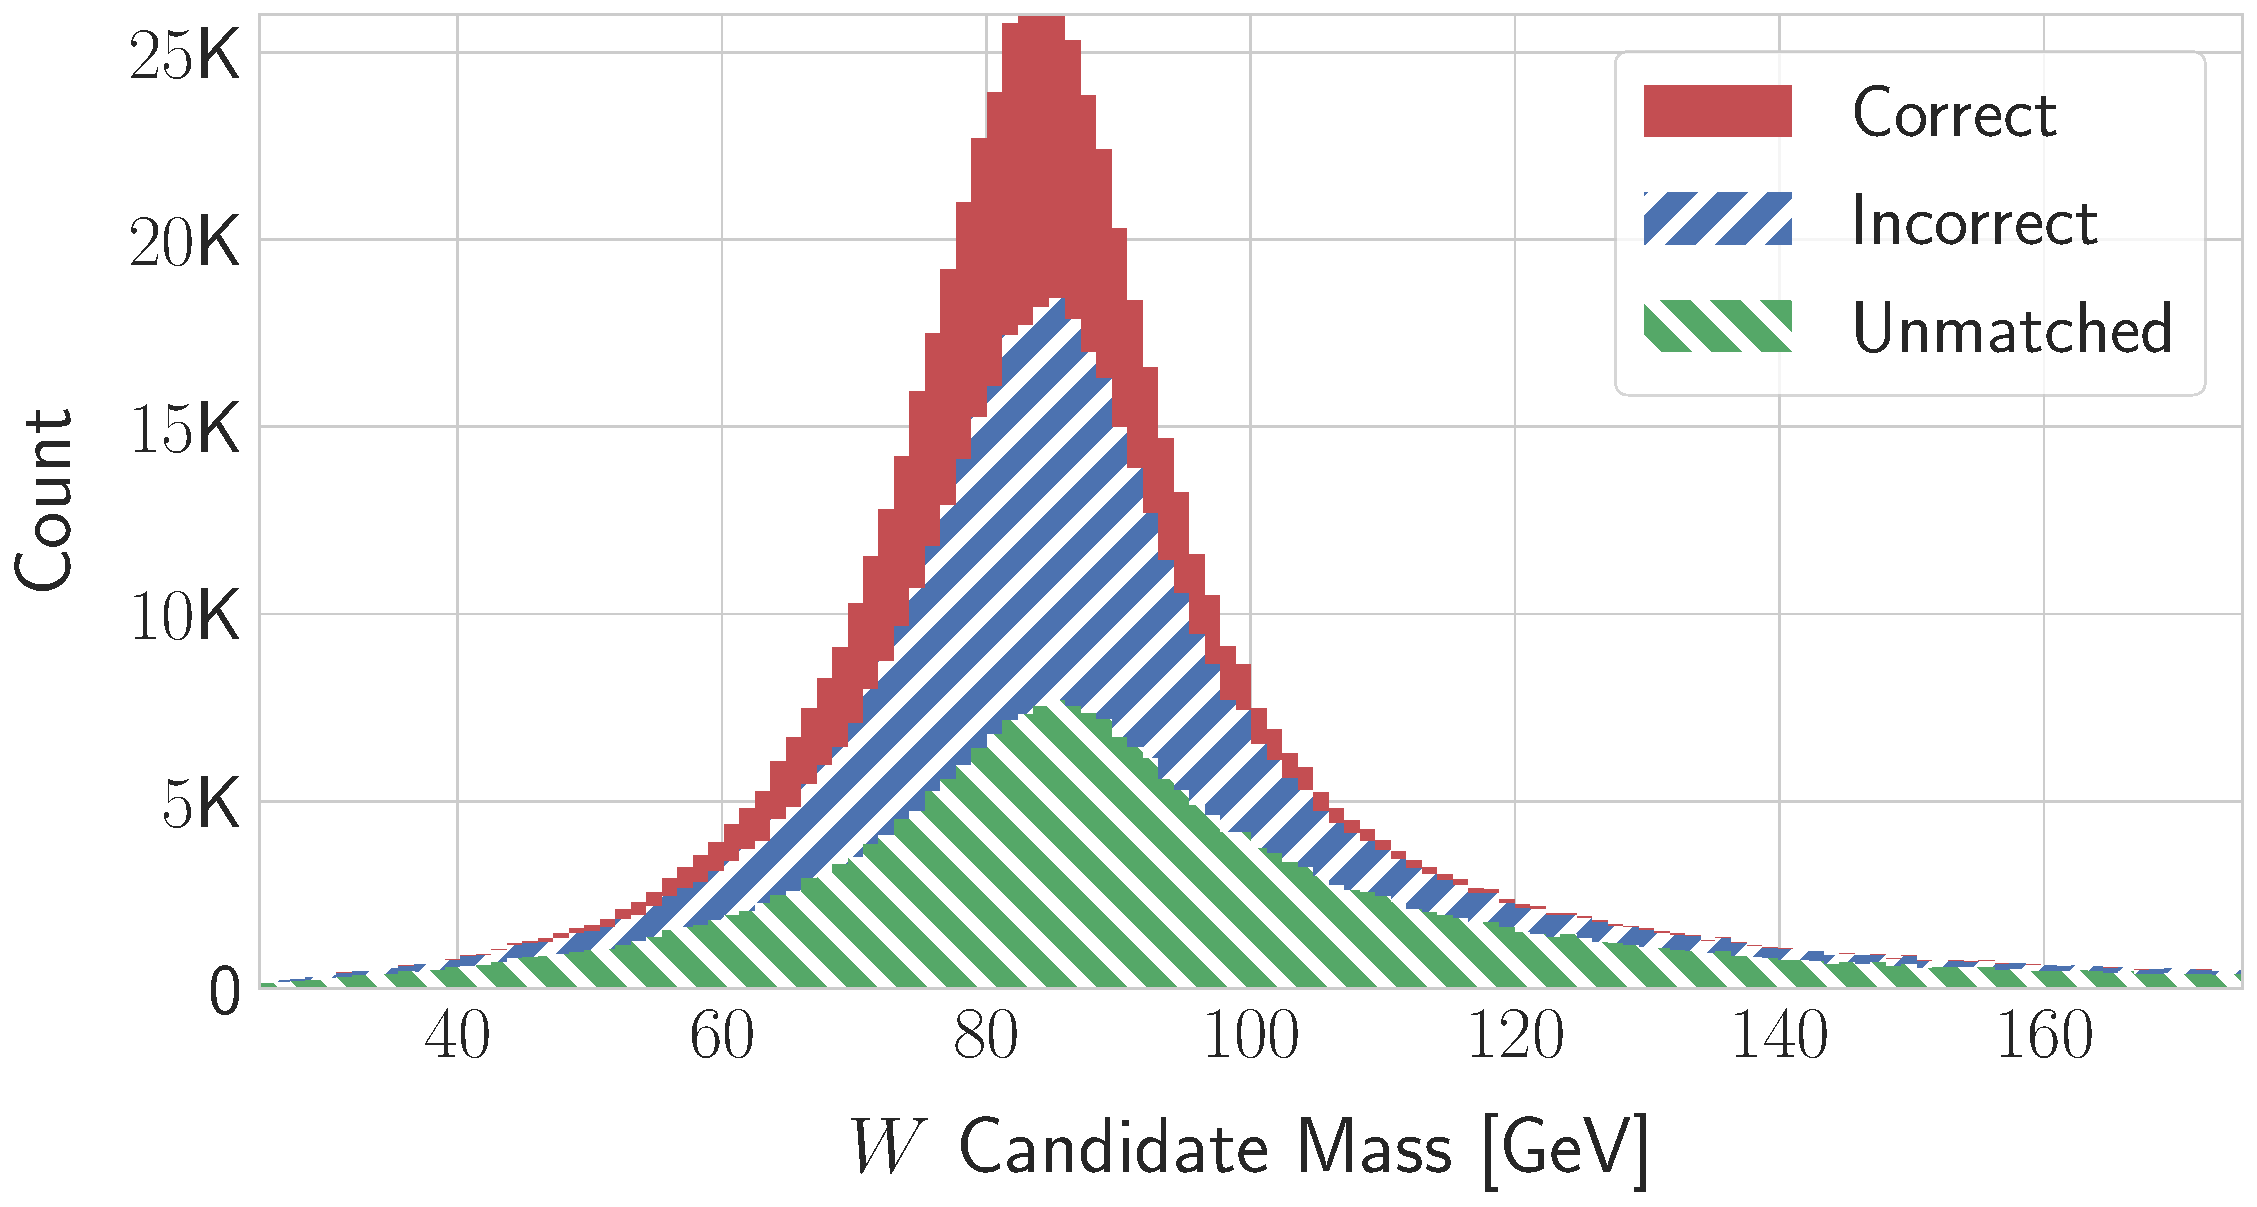
\includegraphics[width=0.7\textwidth]{Figures/network_w_quark_stacked_chi2.pdf}
	\caption{W boson mass reconstructed by $\chi^{2}$ minimization method}
	\label{fig: chi2 reco Wboson}
\end{figure}
\begin{figure}[H]
	\centering
	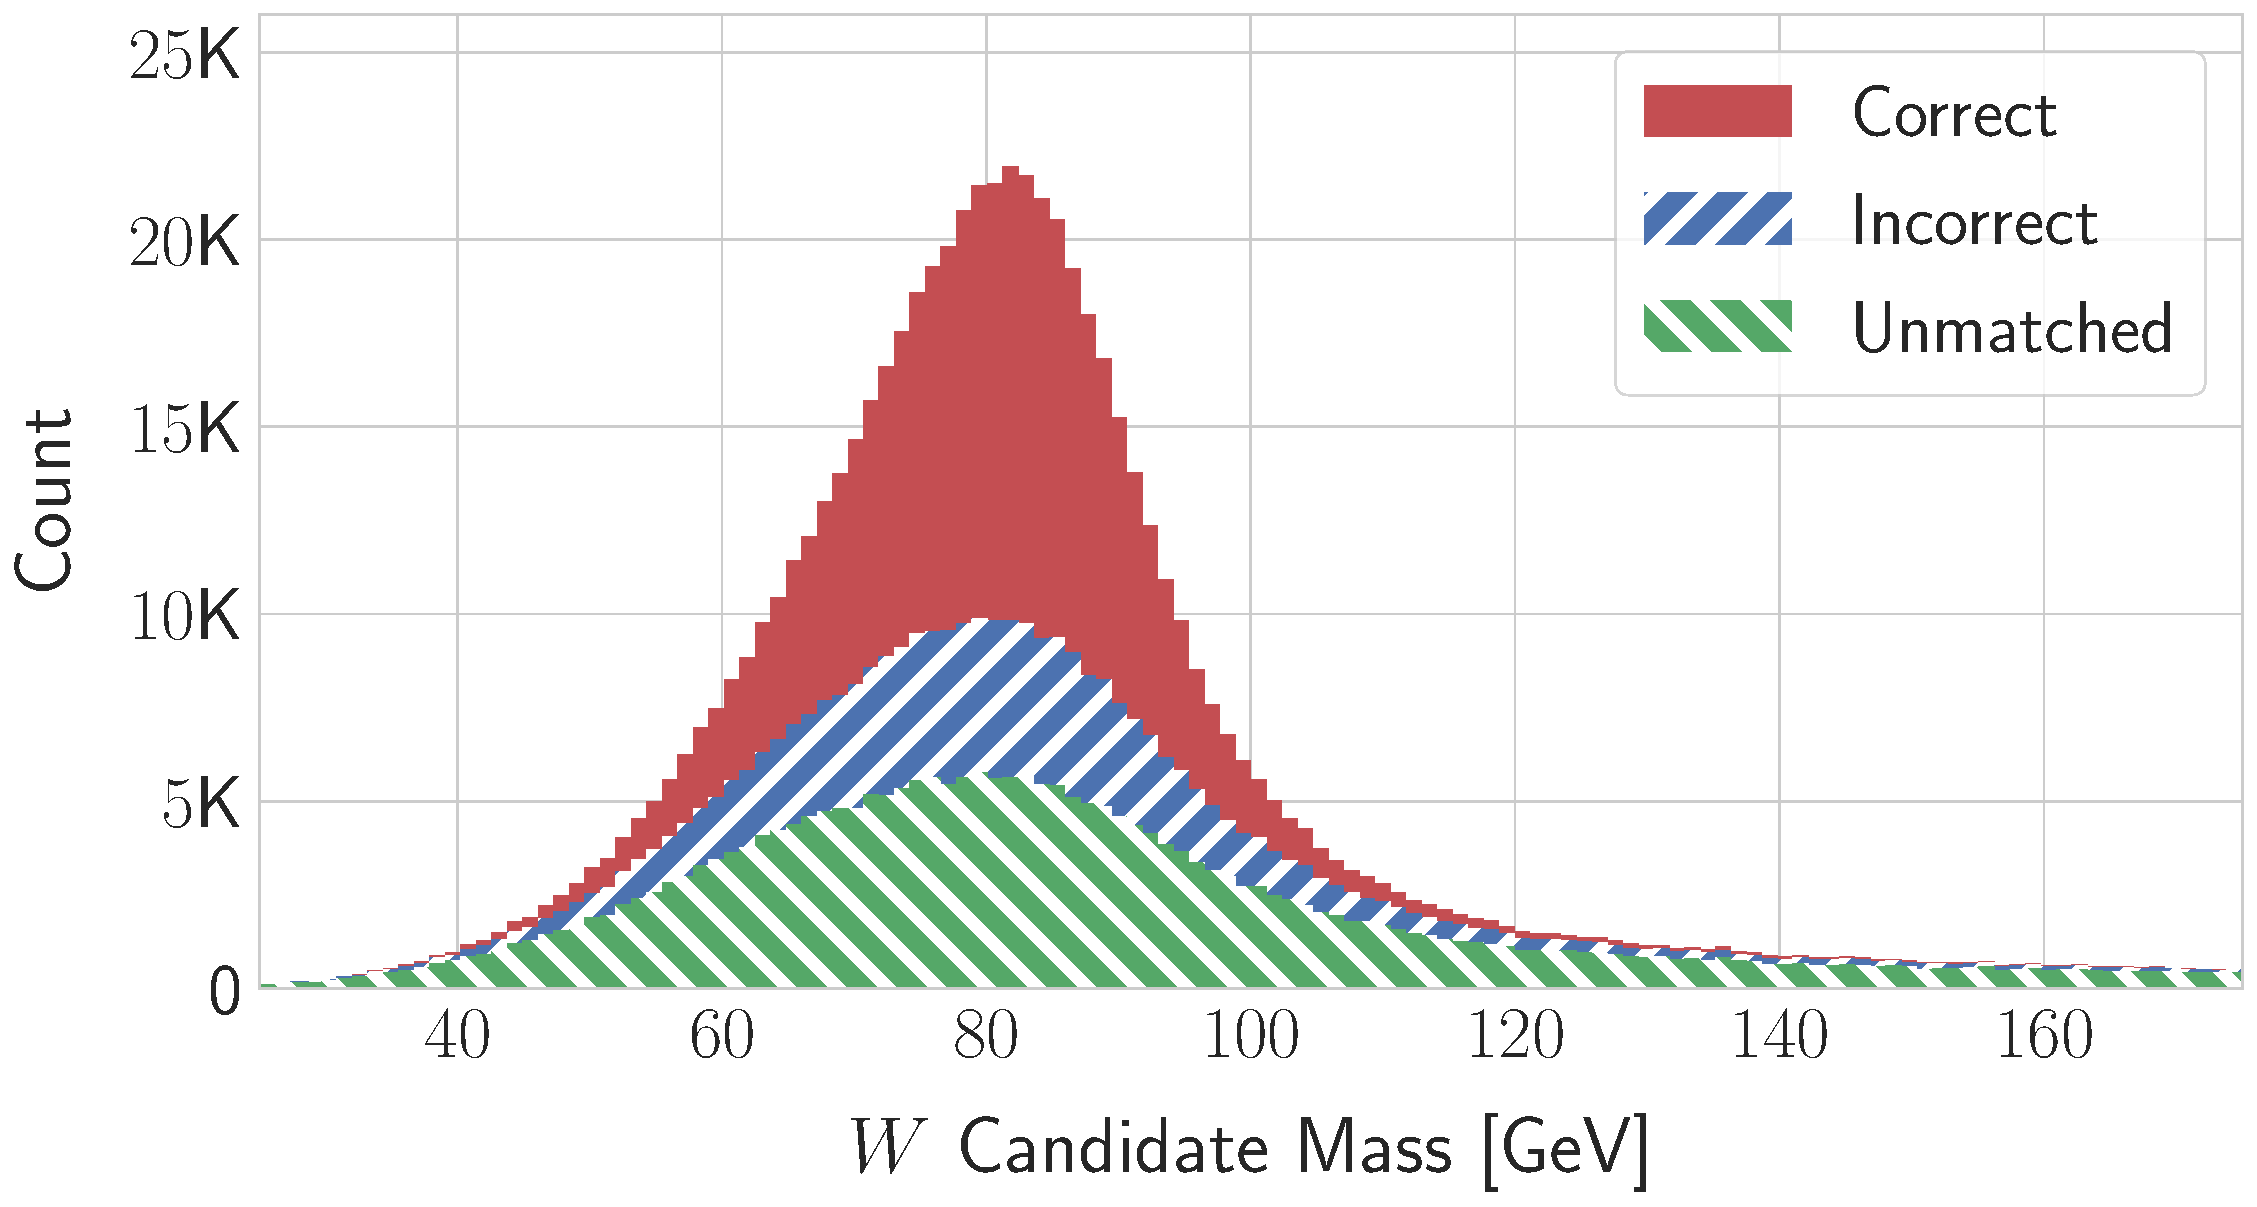
\includegraphics[width=0.7\textwidth]{Figures/network_w_quark_stacked.pdf}
	\caption{W boson mass reconstructed by SPA-NET}
	\label{fig: spanet reco Wboson}
\end{figure}

\begin{figure}[H]
	\centering
	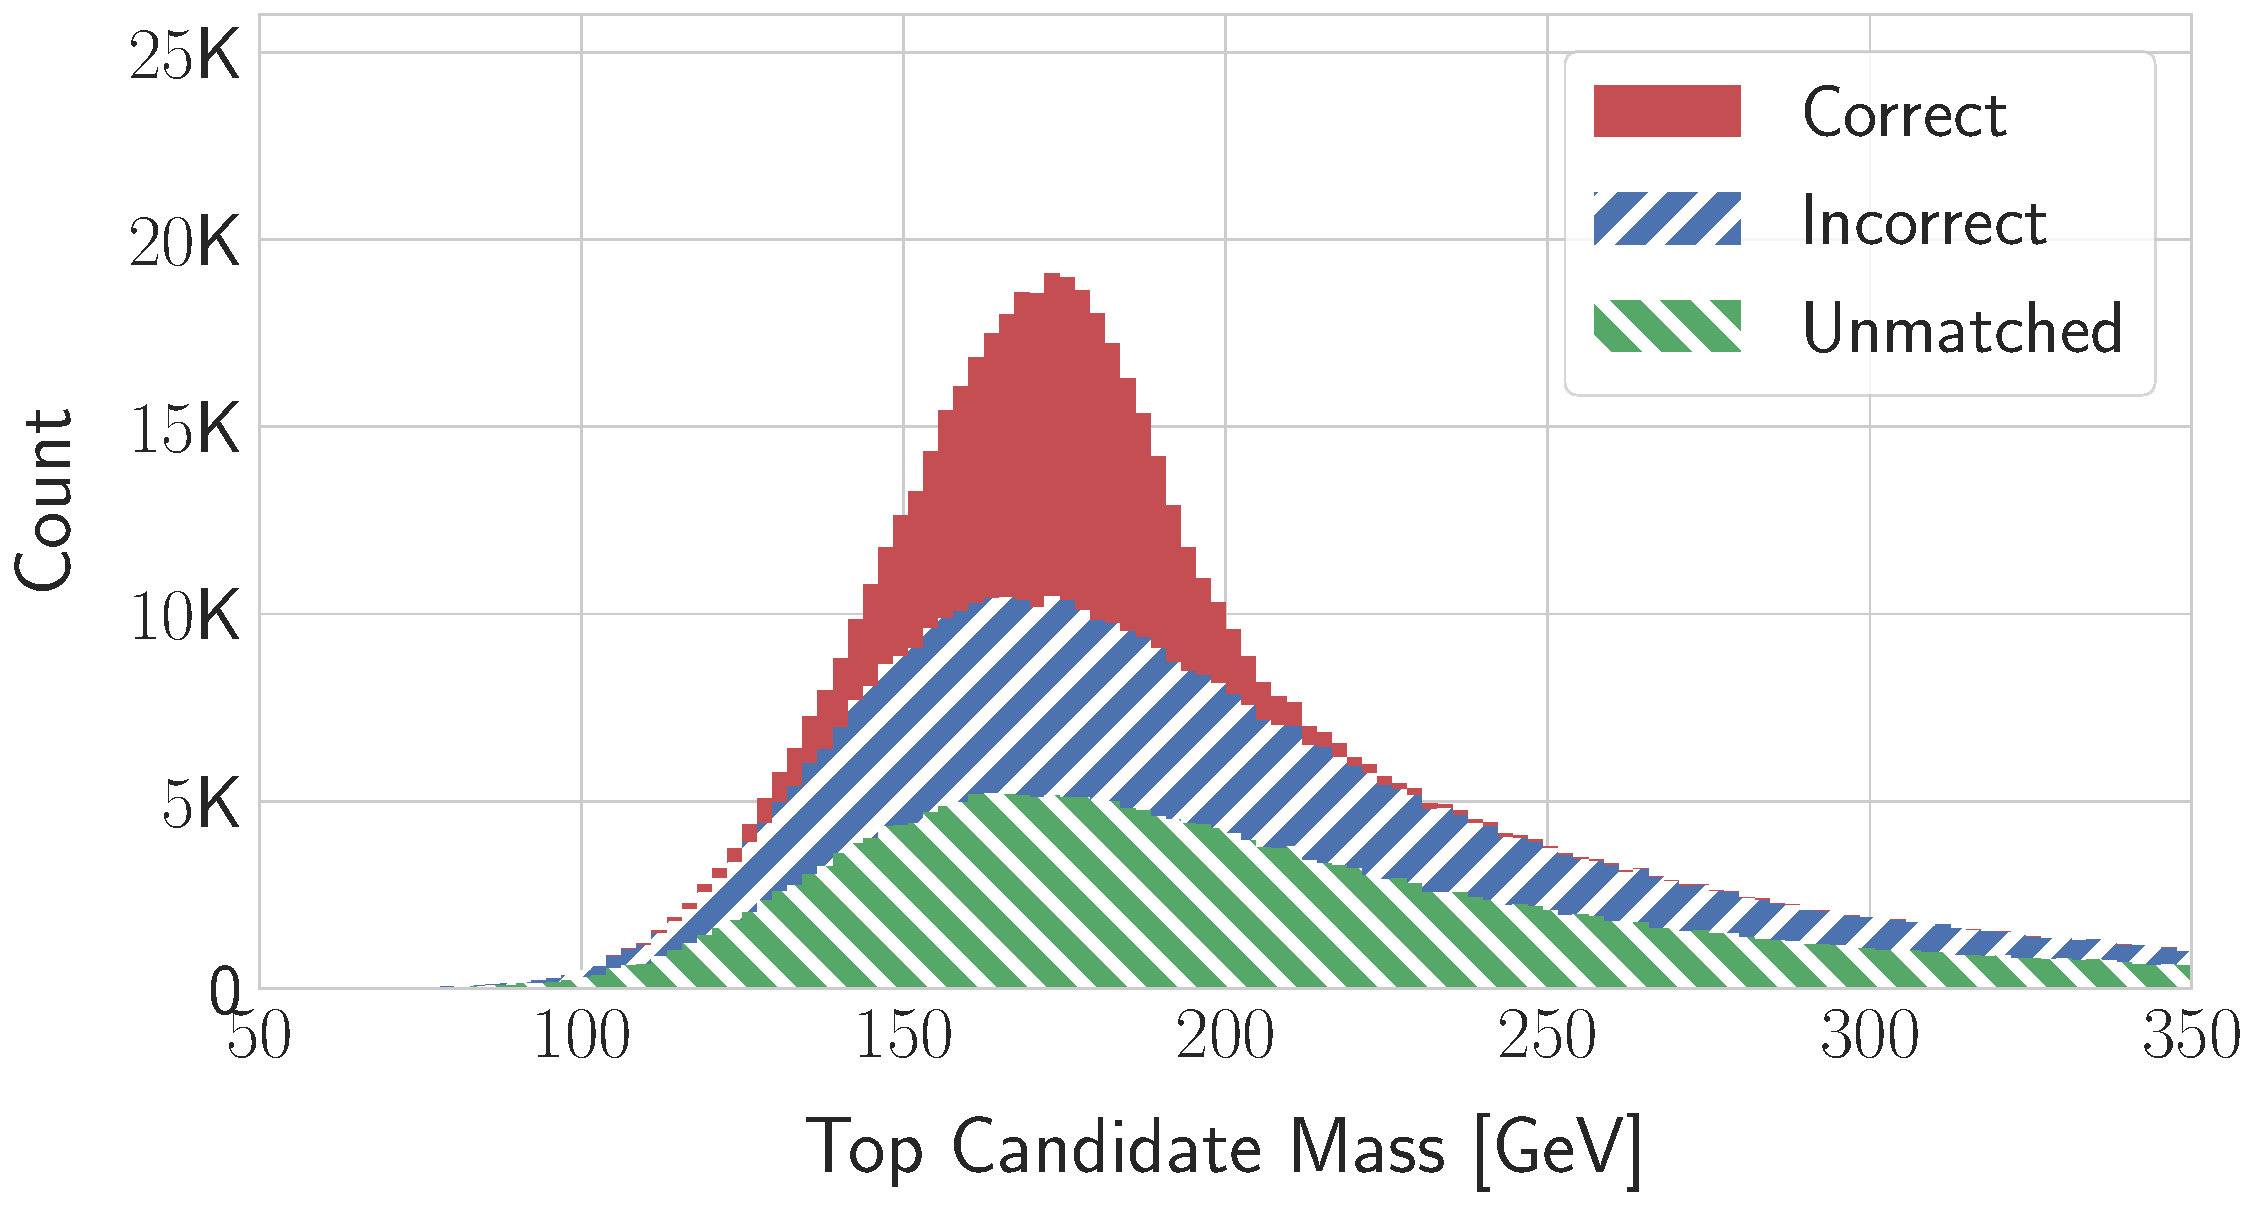
\includegraphics[width=0.7\textwidth]{Figures/network_t_quark_stacked_chi2.pdf}
	\caption{ Top quark mass reconstructed by $\chi^{2}$ minimization method}
	\label{fig: chi2 reco t quark}
\end{figure}
\begin{figure}[H]
	\centering
	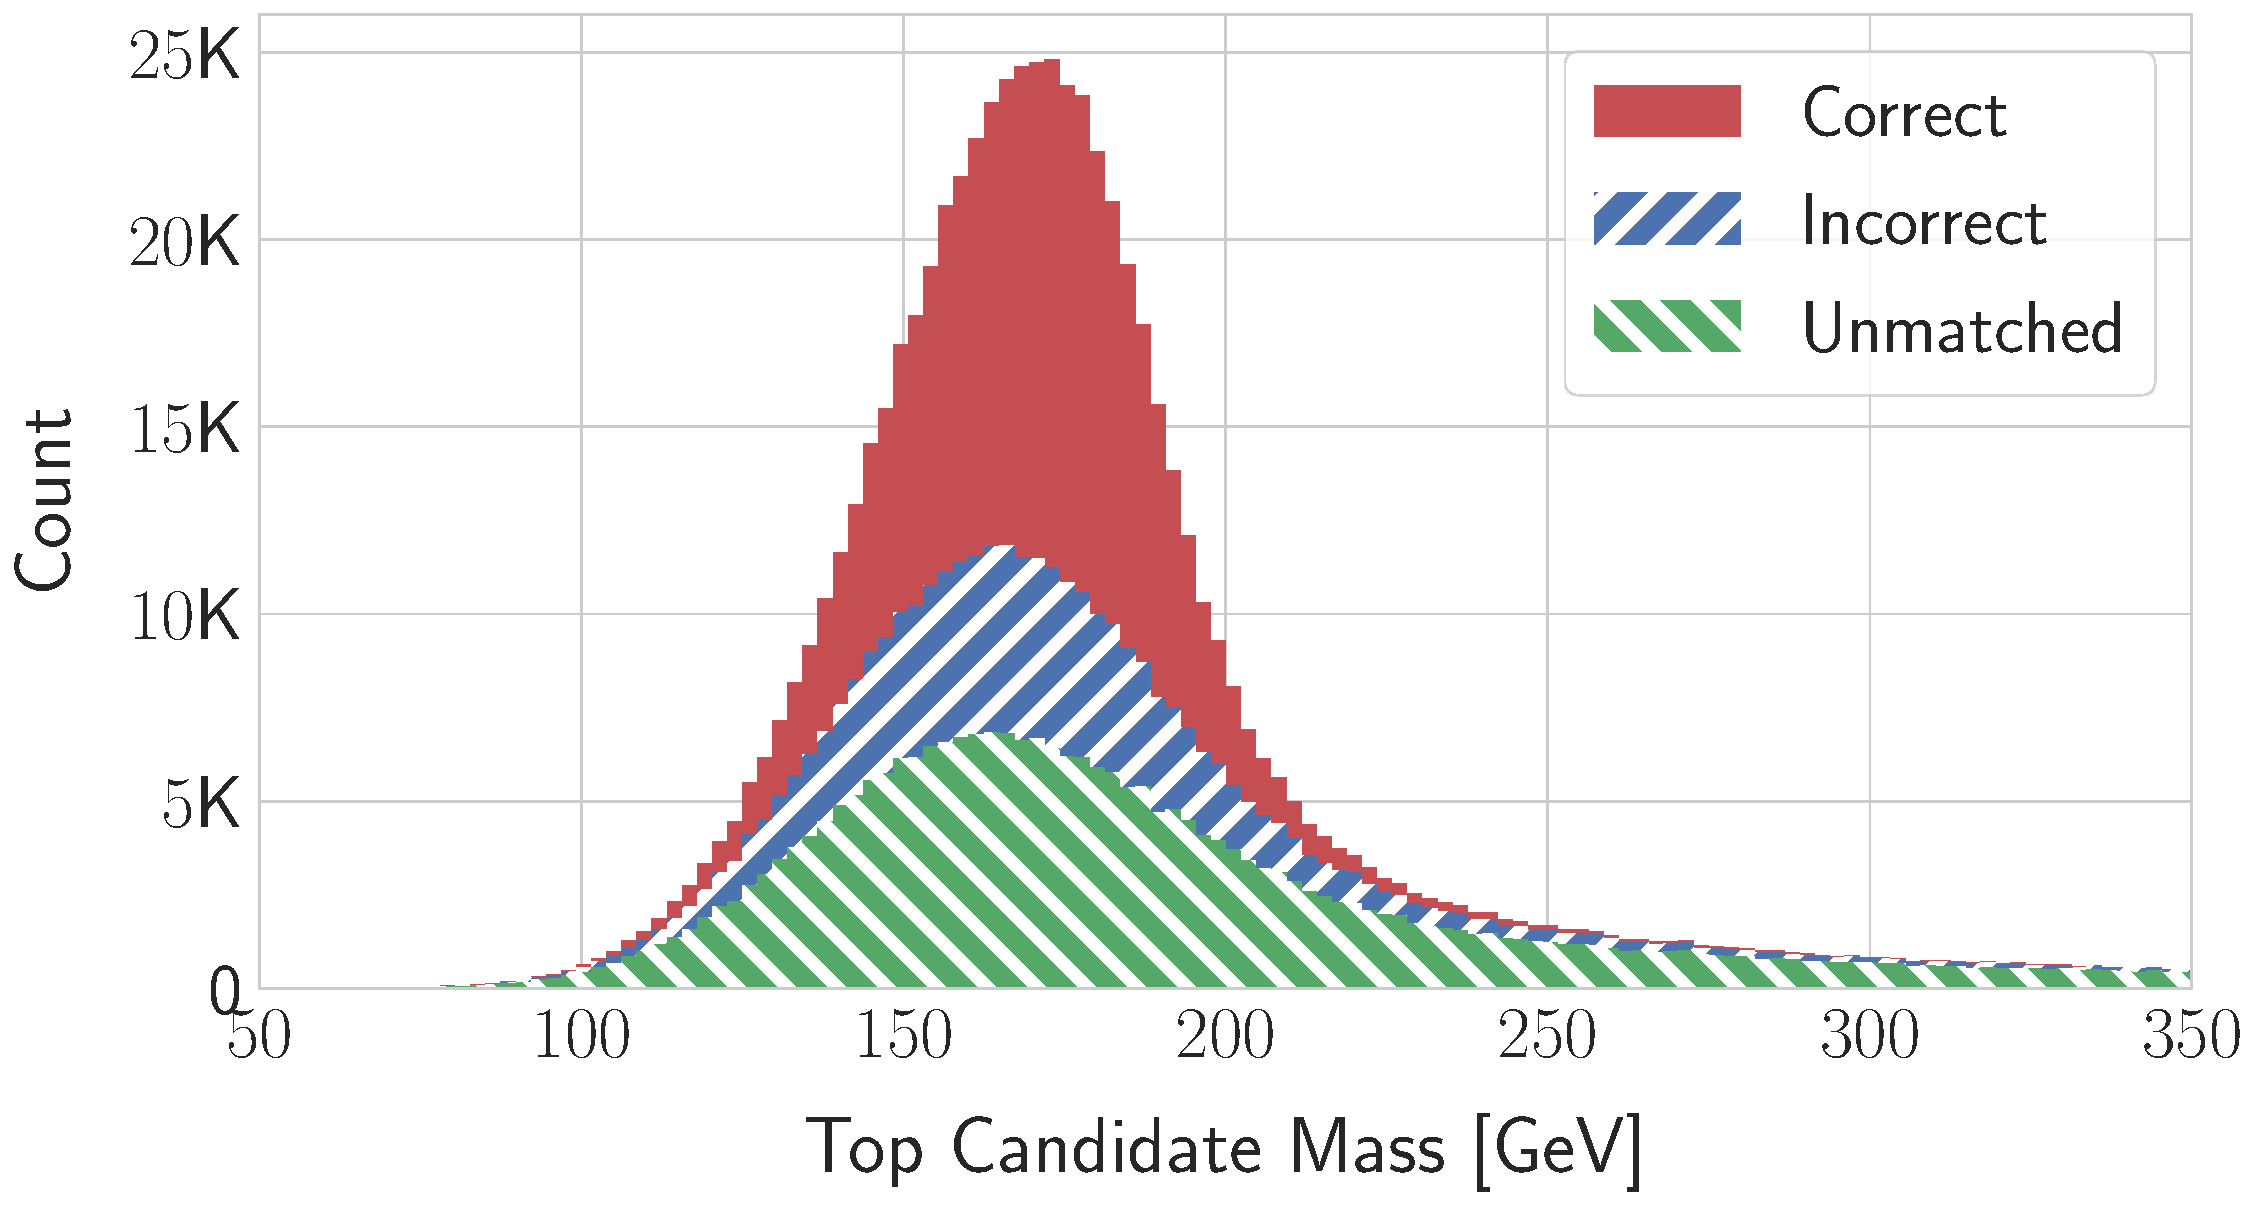
\includegraphics[width=0.7\textwidth]{Figures/network_t_quark_stacked.pdf}
	\caption{ Top quark mass reconstructed by SPA-NET}
	\label{fig: spanet reco t quark}
\end{figure}
Comparing the result shown in Figure \ref{fig: chi2 reco Wboson} and Figure \ref{fig: spanet reco Wboson}, we found the $\chi^{2}$ method has a narrow peak around W boson mass than the SPA-NET. This shape comes from the incorrect and unmatched events and can be explained by the presence of $m_{W}$ in equation \ref{eqn:chi2}. Another point is the Figure \ref{fig: spanet reco t quark} and Figure \ref{fig: chi2 reco t quark} shows that the SPA-NET has the more peaked distribution compare to $\chi^{2}$ method with comparable incorrect/unmatched events.

\subsection{ROC curve}\label{sebsec:roc}

The Receiver operating characteristic (ROC) curve is a good target to estimate the performance of a machine learning model. The ROC curve of SPA-NET apply on events with one and two reconstructable top quarks is shown in Figure \ref{fig: roc one top} and Figure \ref{fig: roc two top}. Note that the targets are defined as 1 if the prediction is correct, otherwise the 0 represents the incorrect prediction.

 \begin{figure}[H]
 	\centering
 	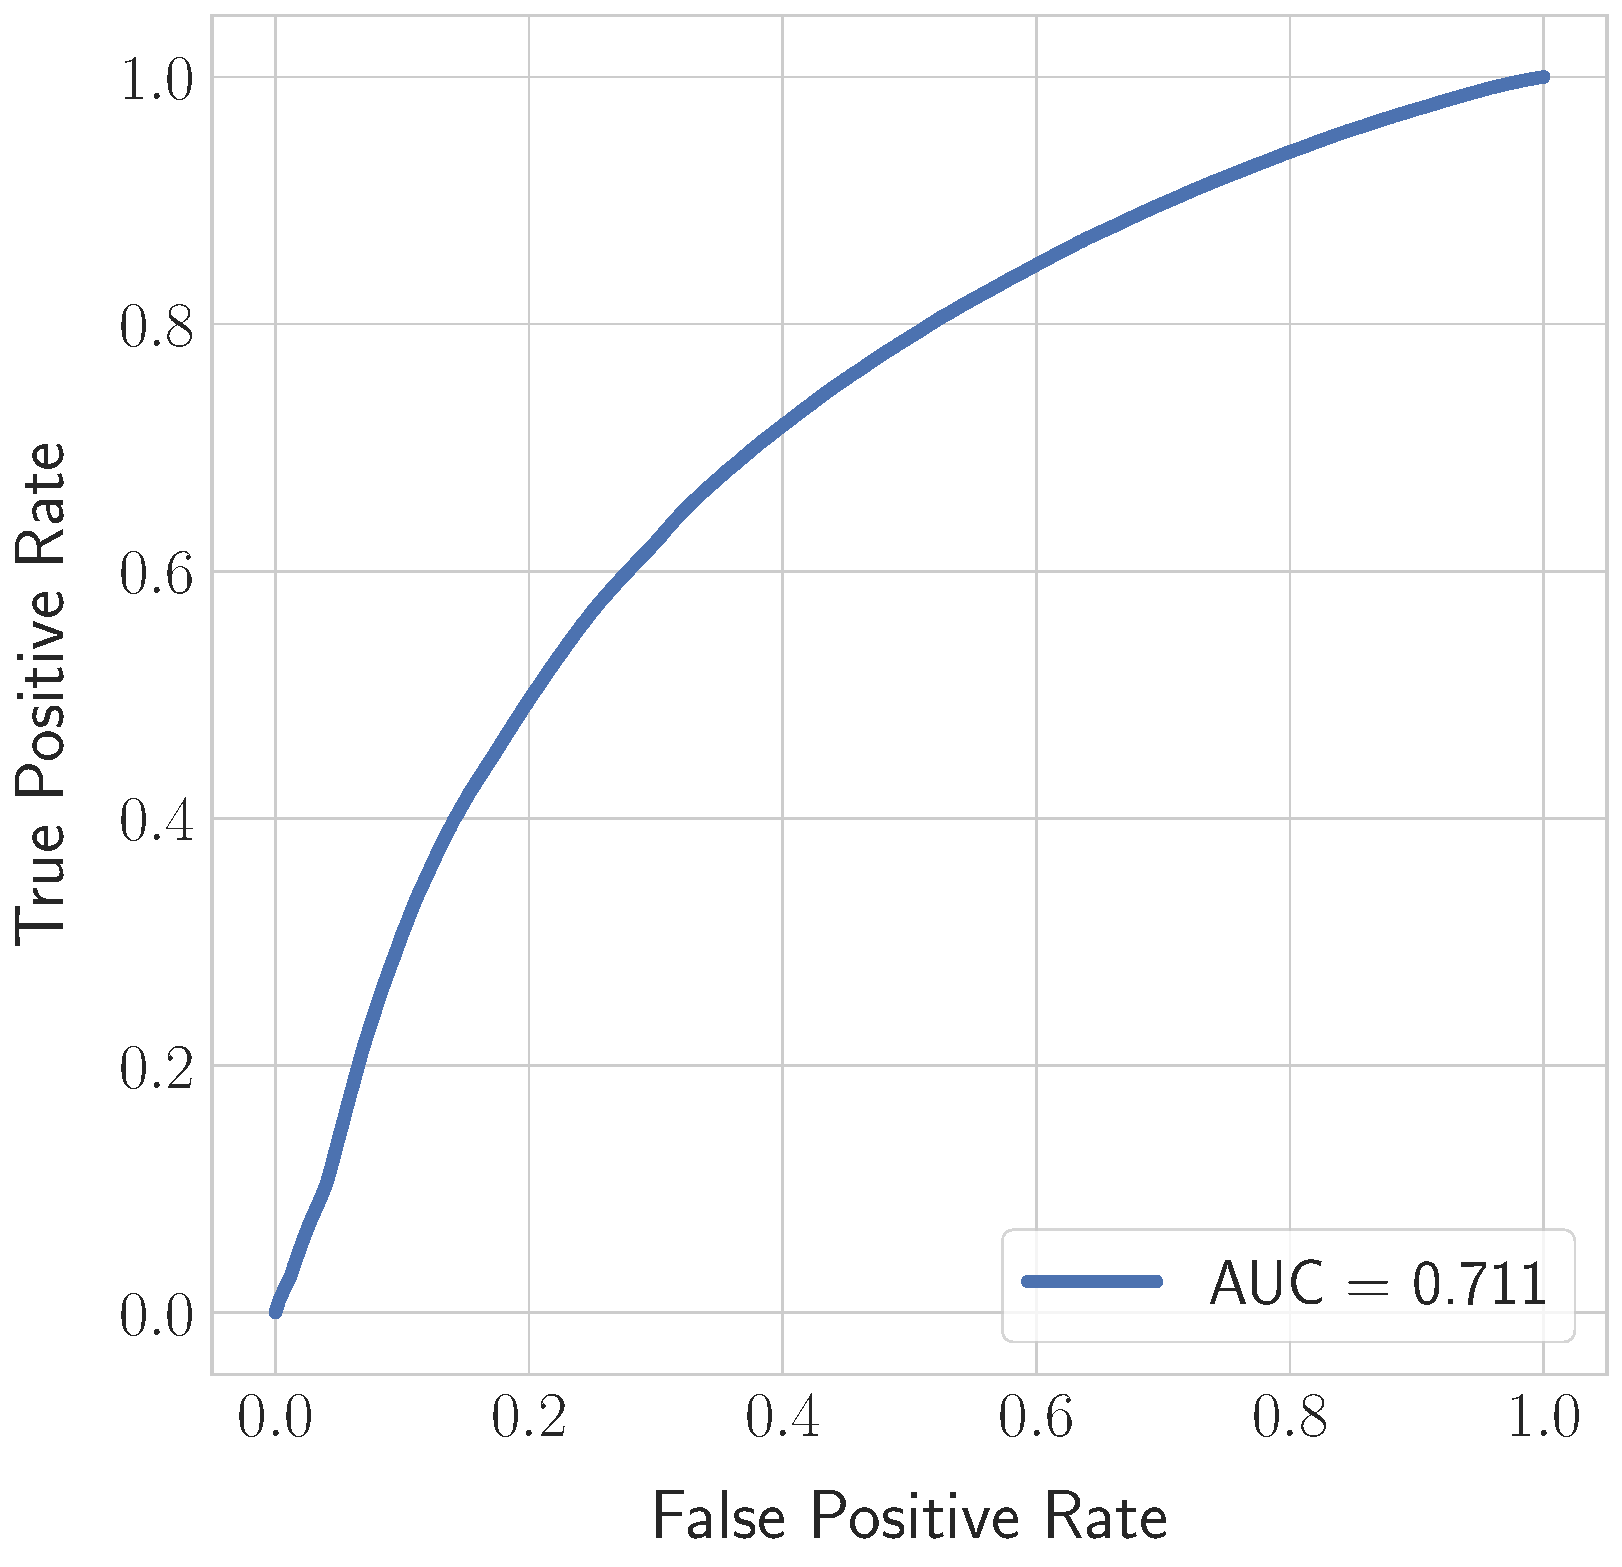
\includegraphics[width=0.6\textwidth]{Figures/roc_one_quark.pdf}
 	\caption{ ROC curve of SPA-NET apply on events with one reconstructable top.}
 	\label{fig: roc one top}
 \end{figure}
 \begin{figure}[H]
 	\centering
 	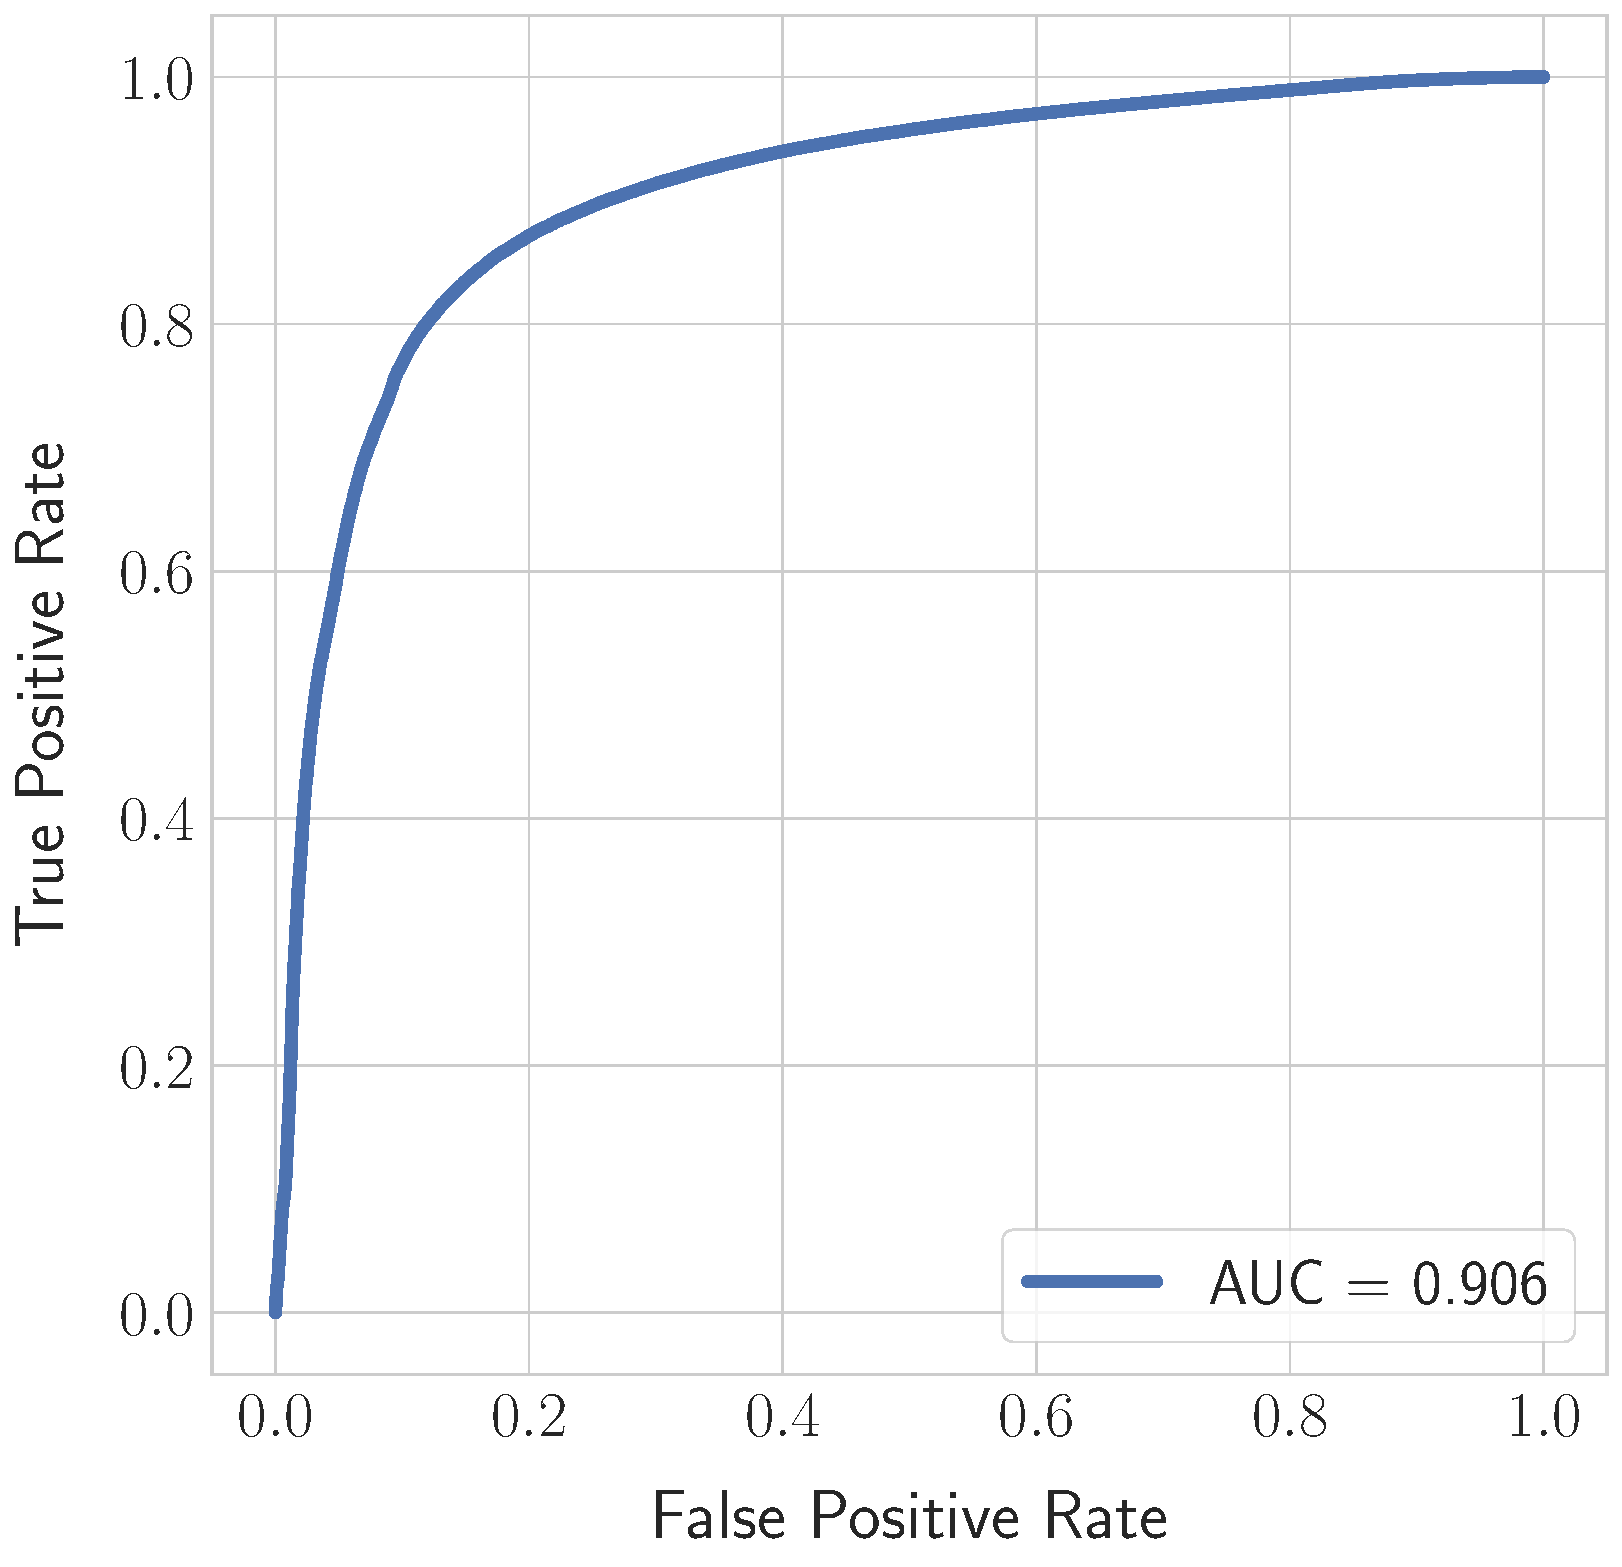
\includegraphics[width=0.6\textwidth]{Figures/roc_two_quark.pdf}
 	\caption{ ROC curve of SPA-NET apply on events with two reconstructable top.}
 	\label{fig: roc two top}
 \end{figure}

\section{Outlook}\label{sec:outlook}

Base on the design of SPA-NET, the input is a sequence of jets information and their relationships. The network considering the permutation relation between each subset and possible permutations. In case, a physics model which has a permutation relationship might be a good target to explore with SPA-NET. For example, $ttH$ all hadronic decay process or all hadronic four top decay process is a potential target to studying with SPA-NET. Further more, not only the parton-jet assignment problem but also the clustering problem, graph matching problem, and so does other problem which contains a permutaion symmetry, is a potential item to study with SPA-NET. We plan to explore the SPA-NET with some interesting BSM problem, such as the tri-Higgs production in 2HDM model.



